%!TEX program = xelatex

\documentclass{beamer}
\usetheme{metropolis}

\setbeamercolor{background canvas}{bg = white}

\usepackage{appendixnumberbeamer}
\renewcommand\appendixname{Appendix}

% packages
\usepackage{amssymb}
\usepackage{amsmath}
\usepackage{mathtools}
\usepackage{hyperref}
\usepackage{lmodern}

% add bibliography
\usepackage[backend = bibtex, style = authoryear, sorting = nyt, dashed = false, natbib]{biblatex}
\renewbibmacro{in:}{}
\addbibresource{bibliography.bib}

% graphics
\graphicspath{ {Figures/} }

% define argmin
\DeclareMathOperator*{\argmin}{arg\,min}

\title{Queues with a Dynamic Schedule}
\author{John Gilbertson}
\date{October 2016}

\begin{document}

\begin{frame}
	\titlepage
\end{frame}

\begin{frame}
	\frametitle{Outline}
	\tableofcontents
\end{frame}

\section{Background}

\begin{frame}
	\frametitle{Queues with Scheduled Arrivals}

	\begin{itemize}
		\item System where customers queue for service
		\item Instead of arriving randomly, customer arrival times are scheduled in advance
		\item Common example is appointments for doctor
		\item Scheduler determines arrival times to minimize expected cost
		\item Expected cost is a linear combination of expected total customers' waiting time and expected server availability time
	\end{itemize}
\end{frame}

\begin{frame}
	\frametitle{Assumptions}

	\begin{itemize}
		\item Single server
		\item Service times are independent exponential RVs with mean $\mu$
		\item All customers arrive punctually
		\item Queue operates on a first in, first out (FIFO) basis
		\item Total number of customers is fixed
	\end{itemize}
\end{frame}

\begin{frame}
	\frametitle{Static vs. Dynamic}

	\begin{itemize}
		\item Static schedules:
		\begin{itemize}
			\item Fixed for the duration of service
		\end{itemize}
		\item Dynamic schedules:
		\begin{itemize}
		 	\item Chosen progressively during service
		 	\item On a customer's arrival, scheduler chooses the next customer's arrival time
		 	\item Reflect ability to reschedule customer arrival times
		 \end{itemize}
		\item Aim to examine the differences between the two schedules
	\end{itemize}
\end{frame}

\begin{frame}
	\frametitle{Literature Review}

	\begin{itemize}
		\item \citet{Bailey} was the first to study such queues
		\item \citet{Pegden} propose a method for finding the optimal static schedule
		\item \citet{Mendel} extends this model to allow for no-shows
		\item \citet{Fiems} include emergency requests that immediately halt the server
		\item \citet{Wang} considers the problem of adding a new customer to a fixed static schedule
	\end{itemize}
\end{frame}

\section{Static Schedules}

\begin{frame}
	\frametitle{Objective Function}

	\begin{itemize}
		\item Denote the expected waiting time of customer $i$ by $w_{i}$
		\begin{equation*}
			\mathbb{E} \Big[ \text{total customers' waiting time} \Big] = \sum_{i = 1}^{n} w_{i}
		\end{equation*}
		\item Denote the interarrival time between customer $i$ and customer $i + 1$ by $x_{i}$
		\begin{equation*}
			\mathbb{E} \Big[ \text{server availability time} \Big] = \sum_{i = 1}^{n - 1} x_{i} + w_{n} + \mu
		\end{equation*}
		\item \alert{Objective function} is a linear combination of these times
		\begin{equation*}
			\phi (\mathbf{x}_{n}) \coloneqq (1 - \gamma) \sum_{i = 1}^{n} w_{i} + \gamma \left( \sum_{i = 1}^{n - 1} x_{i} + w_{n} + \mu \right)
		\end{equation*}
		\item Objective is find $\mathbf{x}_{n}^{*} = (x_{1}^{*}, \ldots, x_{n - 1}^{*})$ to minimise $\phi (\mathbf{x}_{n})$
		\begin{equation*}
			\mathbf{x}_{n}^{*} = \argmin_{\mathbf{x}_{n}} \phi (\mathbf{x}_{n})
		\end{equation*}
	\end{itemize}
\end{frame}

\begin{frame}
	\frametitle{Model for 15 Customers}

	\begin{figure}
			\centering
			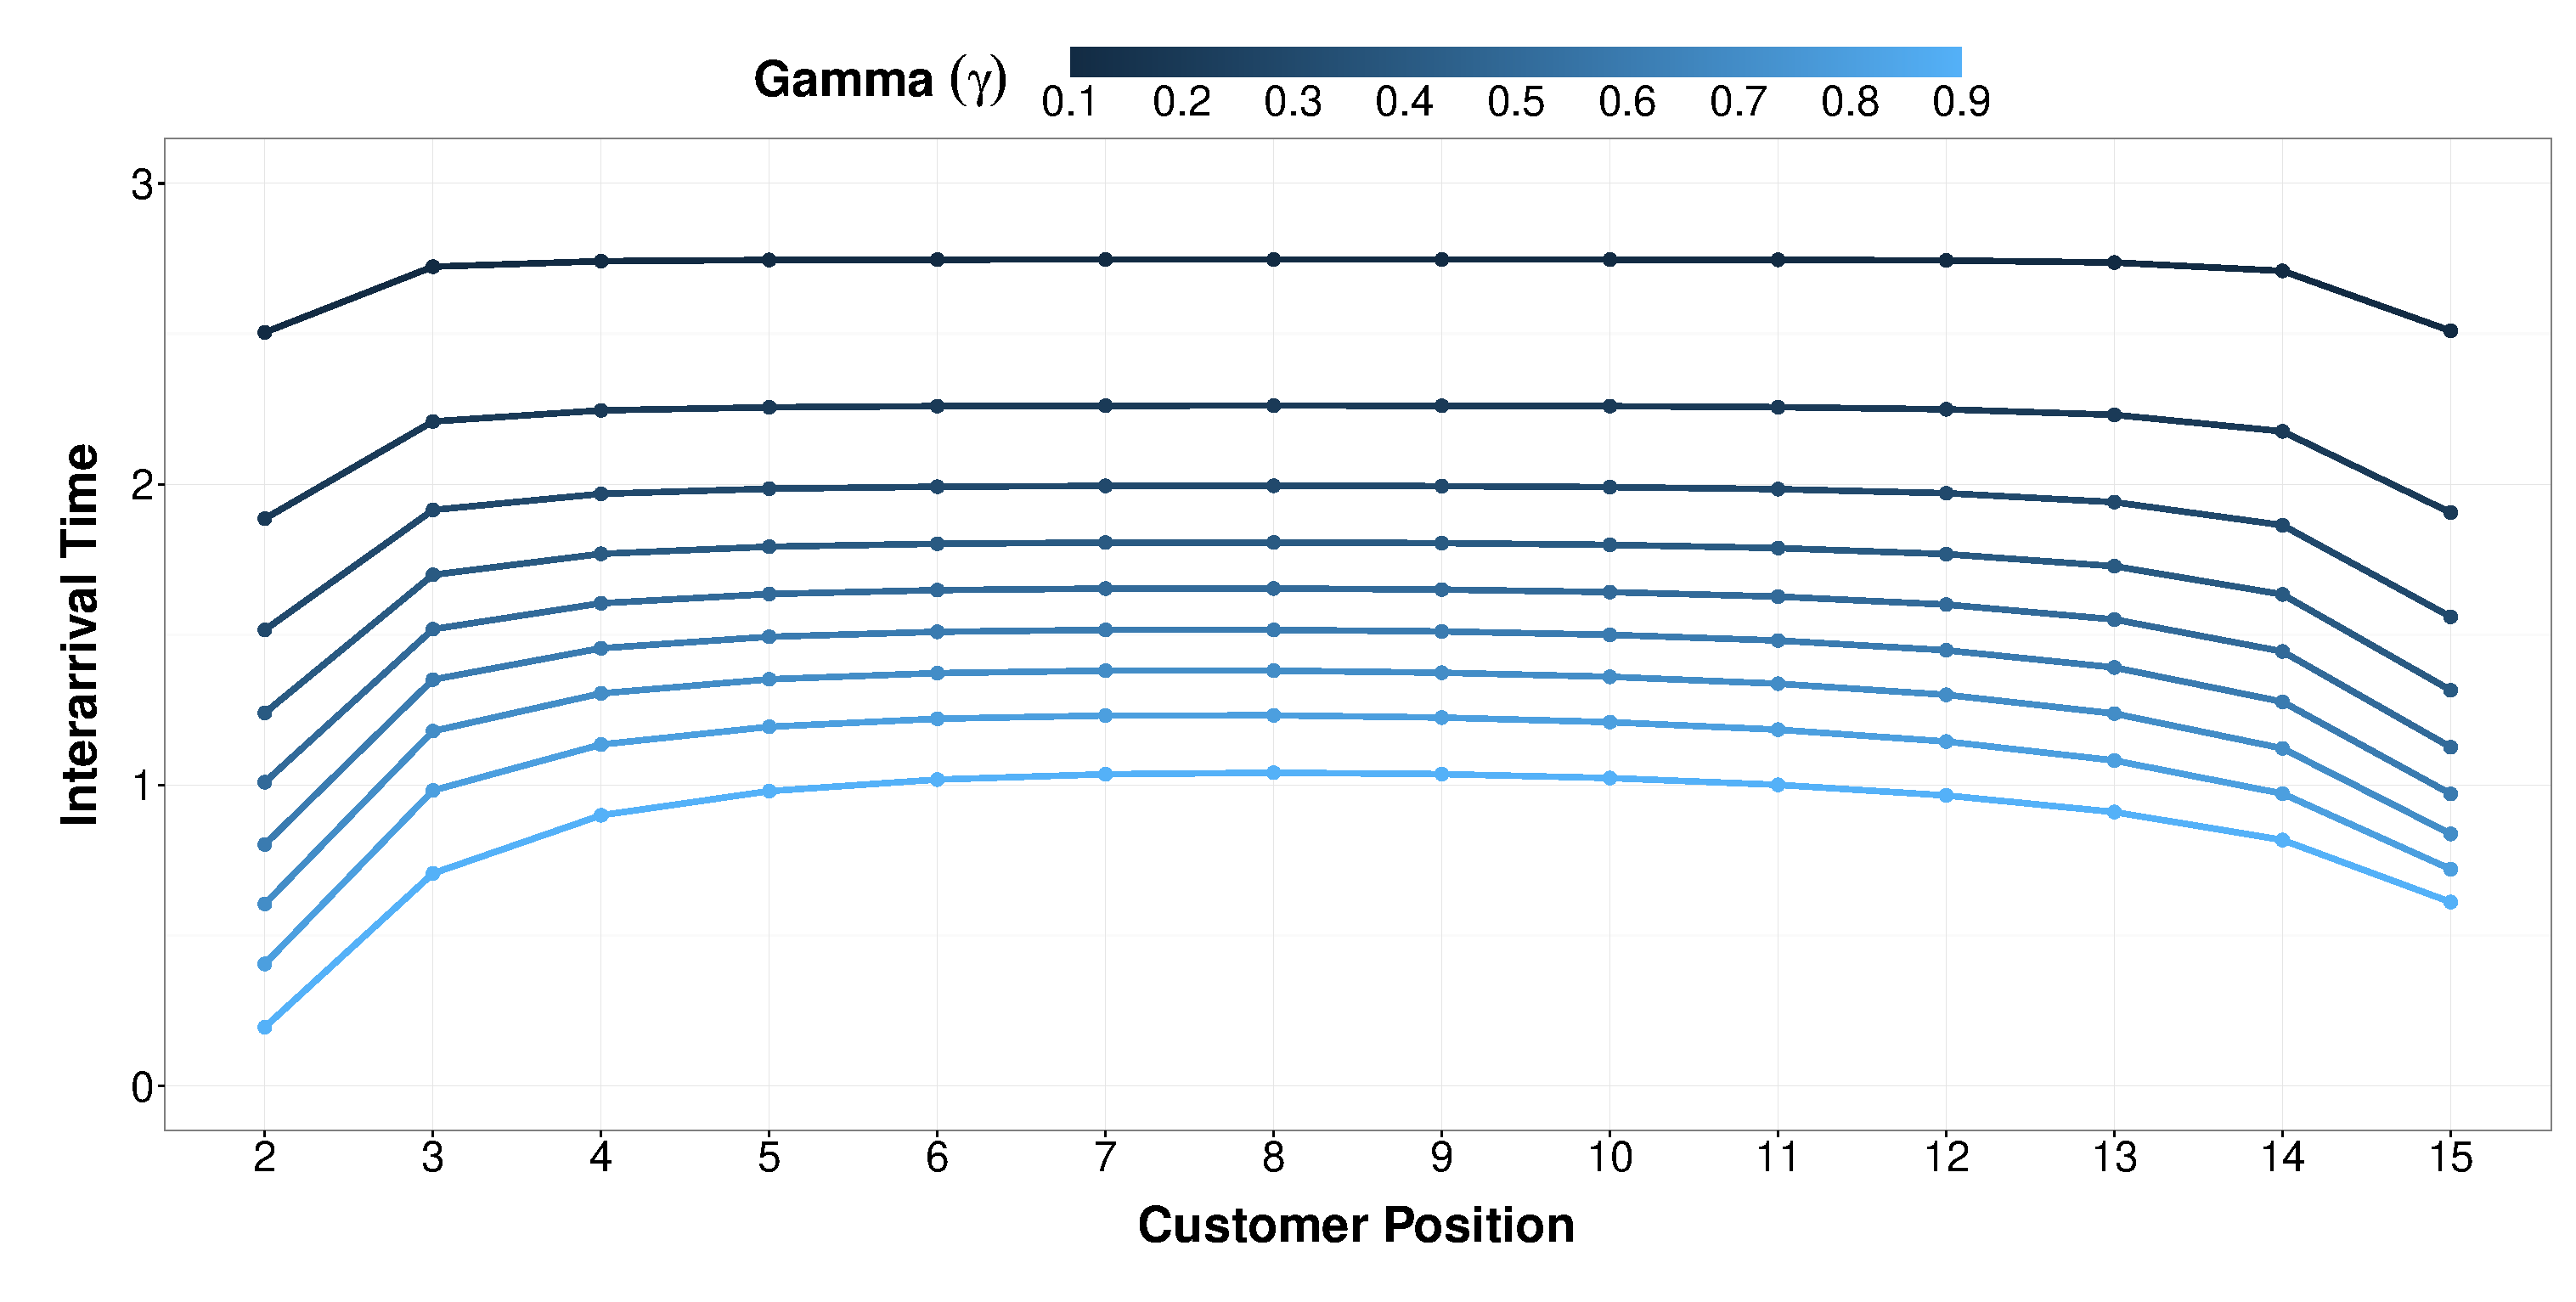
\includegraphics[width=0.85\textwidth]{Static_Line_Interarrival_Gamma.eps}
	\end{figure}

	\begin{itemize}
		\item \alert{Dome-shape}: increase for first customers, remain constant, then decrease for last few customers
		\item As relative cost of server availability time ($\gamma$) increases, customers arrive earlier
	\end{itemize}
\end{frame}

\section{Dynamic Schedules}

\begin{frame}
	\frametitle{Dynamic Schedules}

	\begin{itemize}
		\item Static schedules are fixed for the duration of service
		\item Could be advantageous to allow schedule to vary during service
		\item Dynamic schedule is chosen progressively during service
		\item Arrival of customer $i$ is scheduled on arrival of customer $i - 1$
	\end{itemize}
\end{frame}

\begin{frame}
	\frametitle{Markov Decision Process}

	\begin{itemize}
		\item Consider the problem of scheduling $N$ customers
		\item Denote the number of customers in the system on arrival of customer $i$ by $k_{i}$
		\item $\{ k_{1}, \ldots, k_{N} \}$ is a discrete-time Markov chain
		\item On each customer's arrival, scheduler needs to schedule the arrival time of the next customer denoted by $a$
		\item Set of possible times is $\mathcal{A} = [0, \infty)$
		\item Naturally modeled as \alert{Markov decision process}
	\end{itemize}
\end{frame}

\begin{frame}
	\frametitle{State Transitions}

	\begin{itemize}
		\item Denote the current state of $n$ customers remaining to be scheduled and $k$ customers currently in the system by $(n, k)$
		\item Initial state: $(N, 0)$
		\item State on arrival of first customer: $(N - 1, k_{1})$
		\item State on arrival of last customer: $(0, k_{N})$
		\item From state $(n, k)$, transition to a state $(n - 1, j)$ where
		\begin{equation*}
			j \in \Big\{ 1, 2, \ldots, k + 1 \Big\}
		\end{equation*}
		\item State transition occurs over time interval $a$
	\end{itemize}
\end{frame}

\begin{frame}
	\frametitle{Expected Cost of Schedule}

	\begin{itemize}
		\item Denote the expected cost of state $(n, k)$ assuming the next customer is scheduled to arrive in $a$ time units by $C_{n} (a, k)$
		\item Optimal policy $a^{*}$ minimises the expected cost
		\begin{equation*}
			C_{n}^{*} (k) = C_{n} (a^{*}, k) = \min_{a \geq 0} C_{n} (a, k)
		\end{equation*}
		\item Probability of each transition denoted by $p_{a} (k, j)$
		\item Expected cost of each transition denoted by $R_{a} (k, j)$
		\item Expected cost of state $(n, k)$ by \alert{Bellman equation}:
		\begin{equation*}
			C_{n}^{*} (k) \coloneqq \min_{a \geq 0} C_{n} (a, k) = \min_{a \geq 0} \left[ \sum_{j = 1}^{k + 1} p_{a} (k, j) \Big( R_{a} (k, j) + C_{n - 1}^{*} (j) \Big) \right]
		\end{equation*}
	\end{itemize}
\end{frame}

\begin{frame}
	\frametitle{Erlang Distribution}

	\begin{itemize}
		\item Waiting time of customer in position $r + 1$ is sum of $r$ independent Exponential RVs with mean $\mu$
		\begin{equation*}
		 	X = \sum_{i = 1}^{r} S_{i} \sim \text{Erlang} (r, \mu)
		\end{equation*}
		\item Distribution function:
		\begin{equation*}
			F (a; r) \coloneqq \mathbb{P} (X \leq x) = \begin{cases} 0 & \text{where $x = 0$} \\ 1 - \sum_{i = 0}^{r - 1} \frac{1}{i!} \left( \frac{x}{\mu} \right)^{i} \mathrm{e}^{\frac{-x}{\mu}} & \text{where $x > 0$} \end{cases}
		\end{equation*}
		\item Conditional expectation:
		\begin{equation*}
			\mathbb{E} \Big[ X \ \big| \ X \leq a \Big] = \mu r \times \frac{F (a; r + 1)}{F (a; r)}
		\end{equation*}
		\item Suppose $Y \sim \text{Exp} (\mu)$ independent of $X$ 
		\begin{equation*}
			\mathbb{E} \Big[ X \ \big| \ X \leq a, X + Y > a \Big] = \frac{a r}{r + 1}
		\end{equation*}
	\end{itemize}
\end{frame}

\begin{frame}
	\frametitle{Model for 15 Customers}

	\begin{figure}
		\centering
		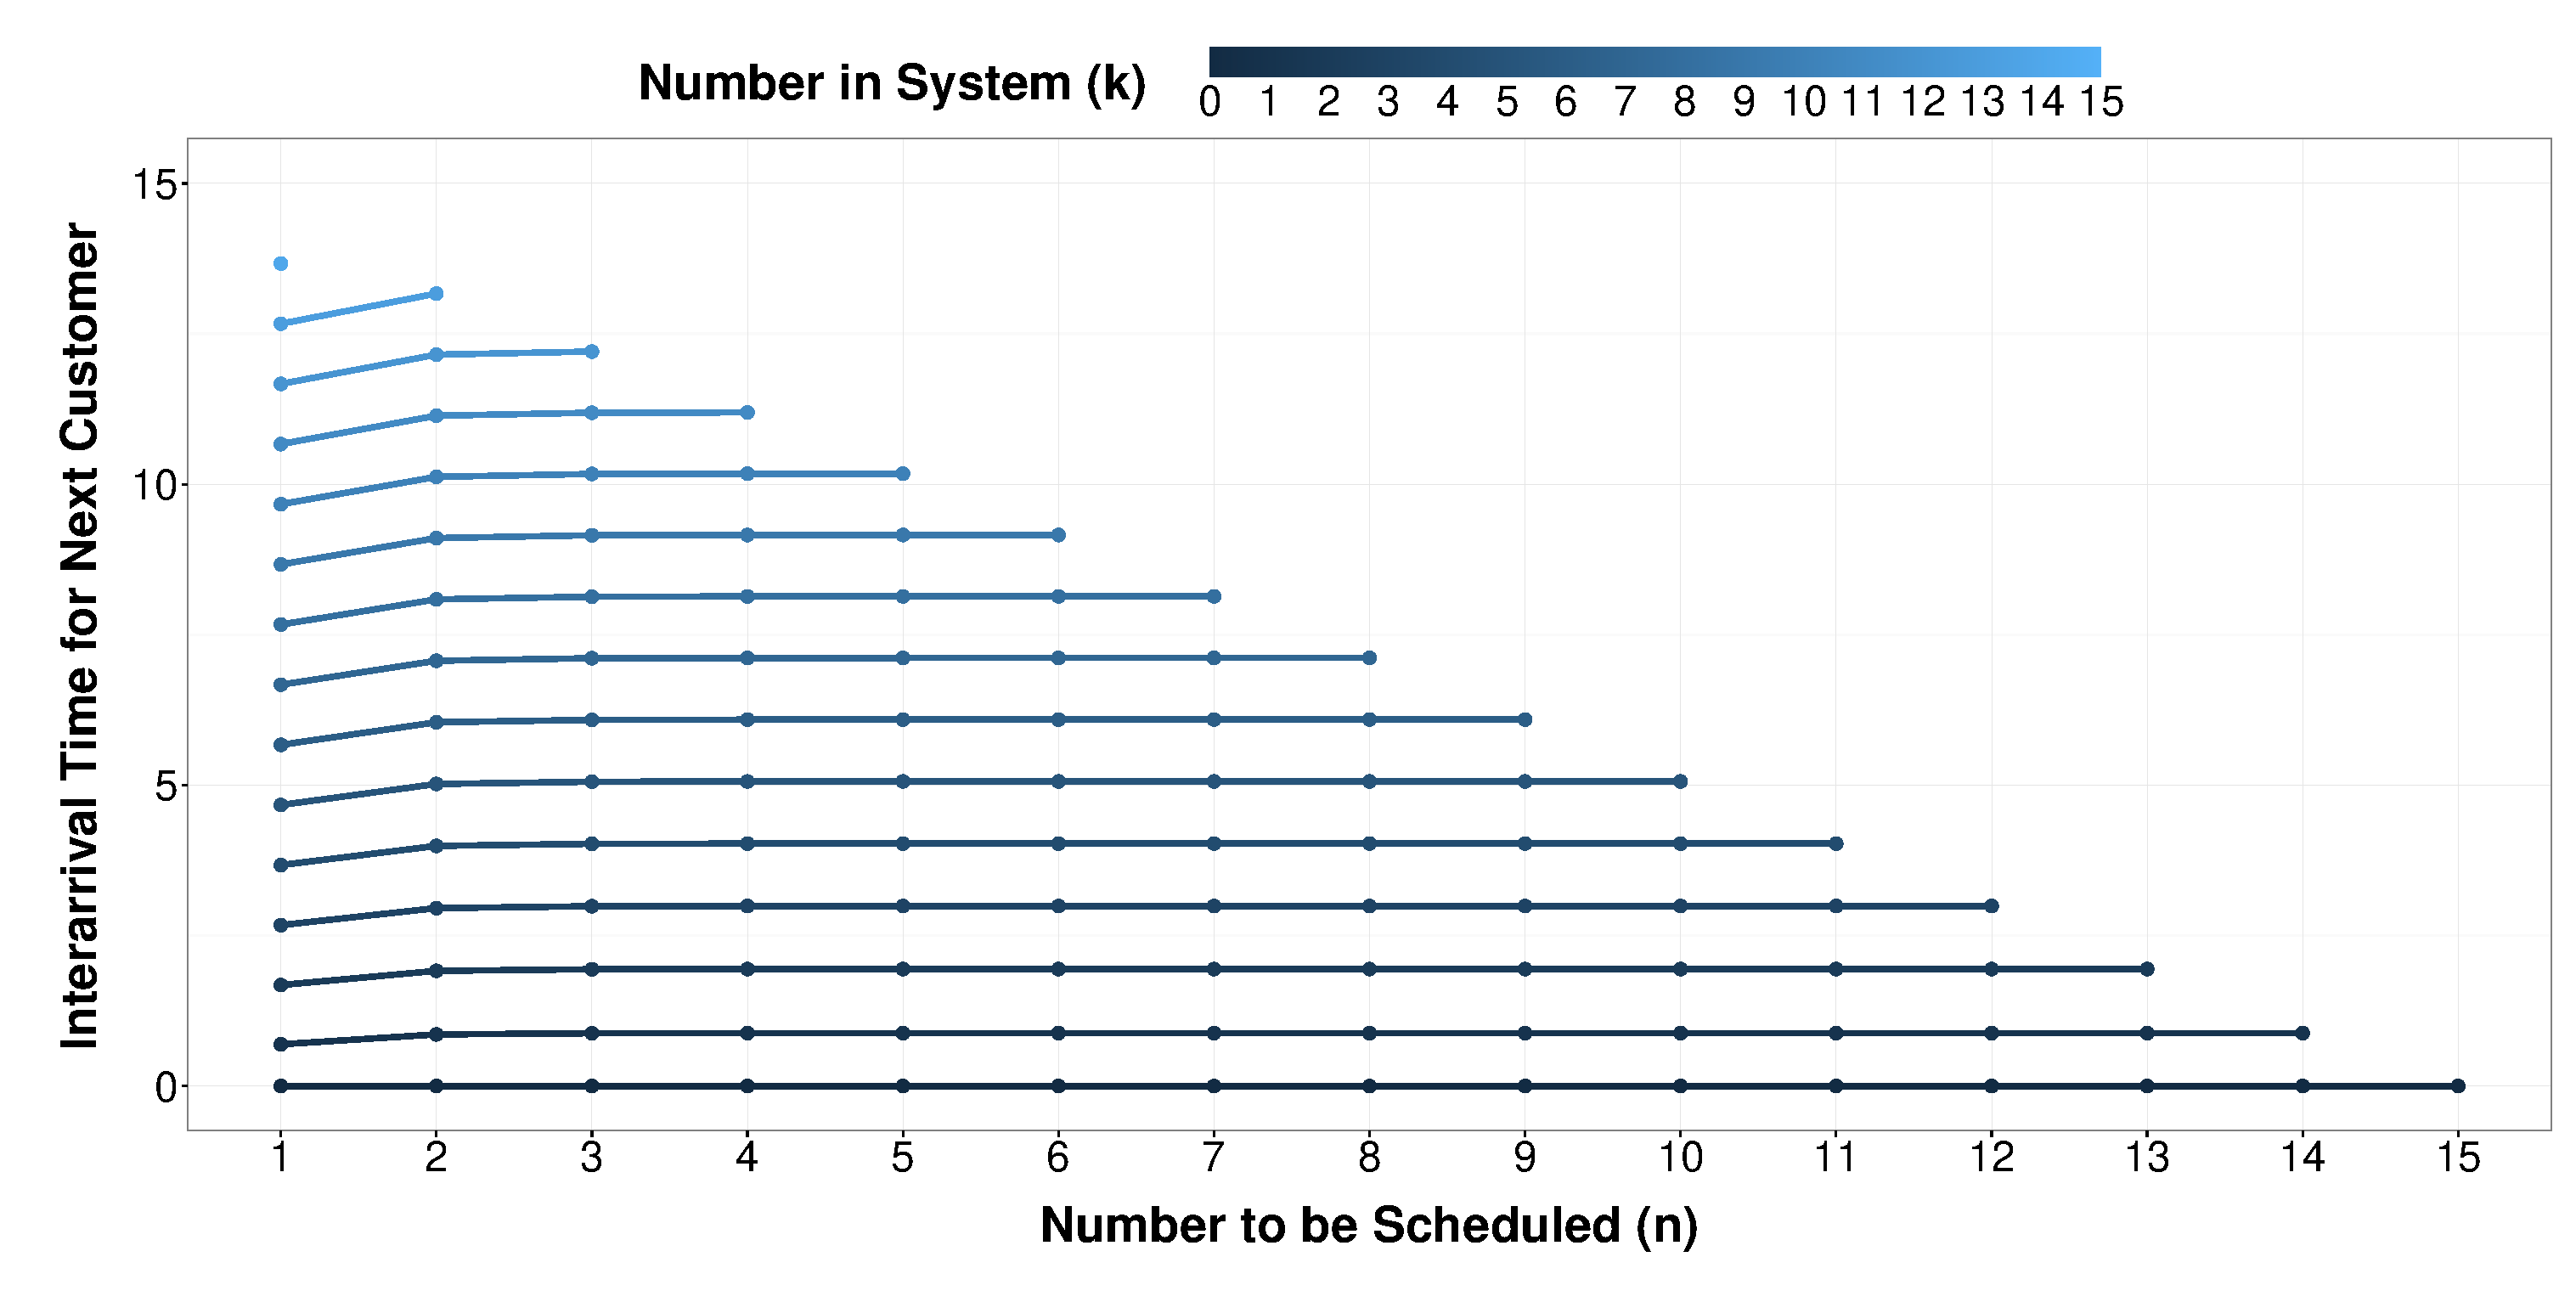
\includegraphics[width=0.85\textwidth]{Dynamic_Line_Interarrival_k.eps}
	\end{figure}

	\begin{itemize}
		\item Plot of optimal interarrival times $a^{*}$ for each possible state
		\item $a^{*} = 0$ for initial state $(15, 0)$, and $a^{*} = 10.17$ for state $(3, 10)$
		\item $a^{*}$ is independent of $n$ for $n \geq 2$
	\end{itemize}
\end{frame}

\section{Schedule Comparison}

\begin{frame}
	\frametitle{Expected Cost Comparison}

	\begin{itemize}
		\item Consider the problem of scheduling $N$ customers
		\item Expected cost of optimal static schedule is $\phi (\mathbf{x}_{N}^{*})$
		\item Expected cost of optimal dynamic schedule is $C_{N}^{*} (0)$
		\item Dynamic schedule is never worse (in expectation):
		\begin{equation*}
			C_{N}^{*} (0) \leq \phi (\mathbf{x}_{N}^{*})
		\end{equation*}
		\item Equality holds for $N \in \{ 0, 1, 2 \}$
		\item Define the \alert{expected percentage cost saving} as
		\begin{equation*}
			\Delta C \coloneqq 100 \times \frac{\phi (\mathbf{x}_{N}^{*}) - C_{N}^{*} (0)}{\phi (\mathbf{x}_{N}^{*})}
		\end{equation*}
	\end{itemize}
\end{frame}

\begin{frame}
	\frametitle{Expected Percentage Cost Saving}

	\begin{figure}
		\centering
		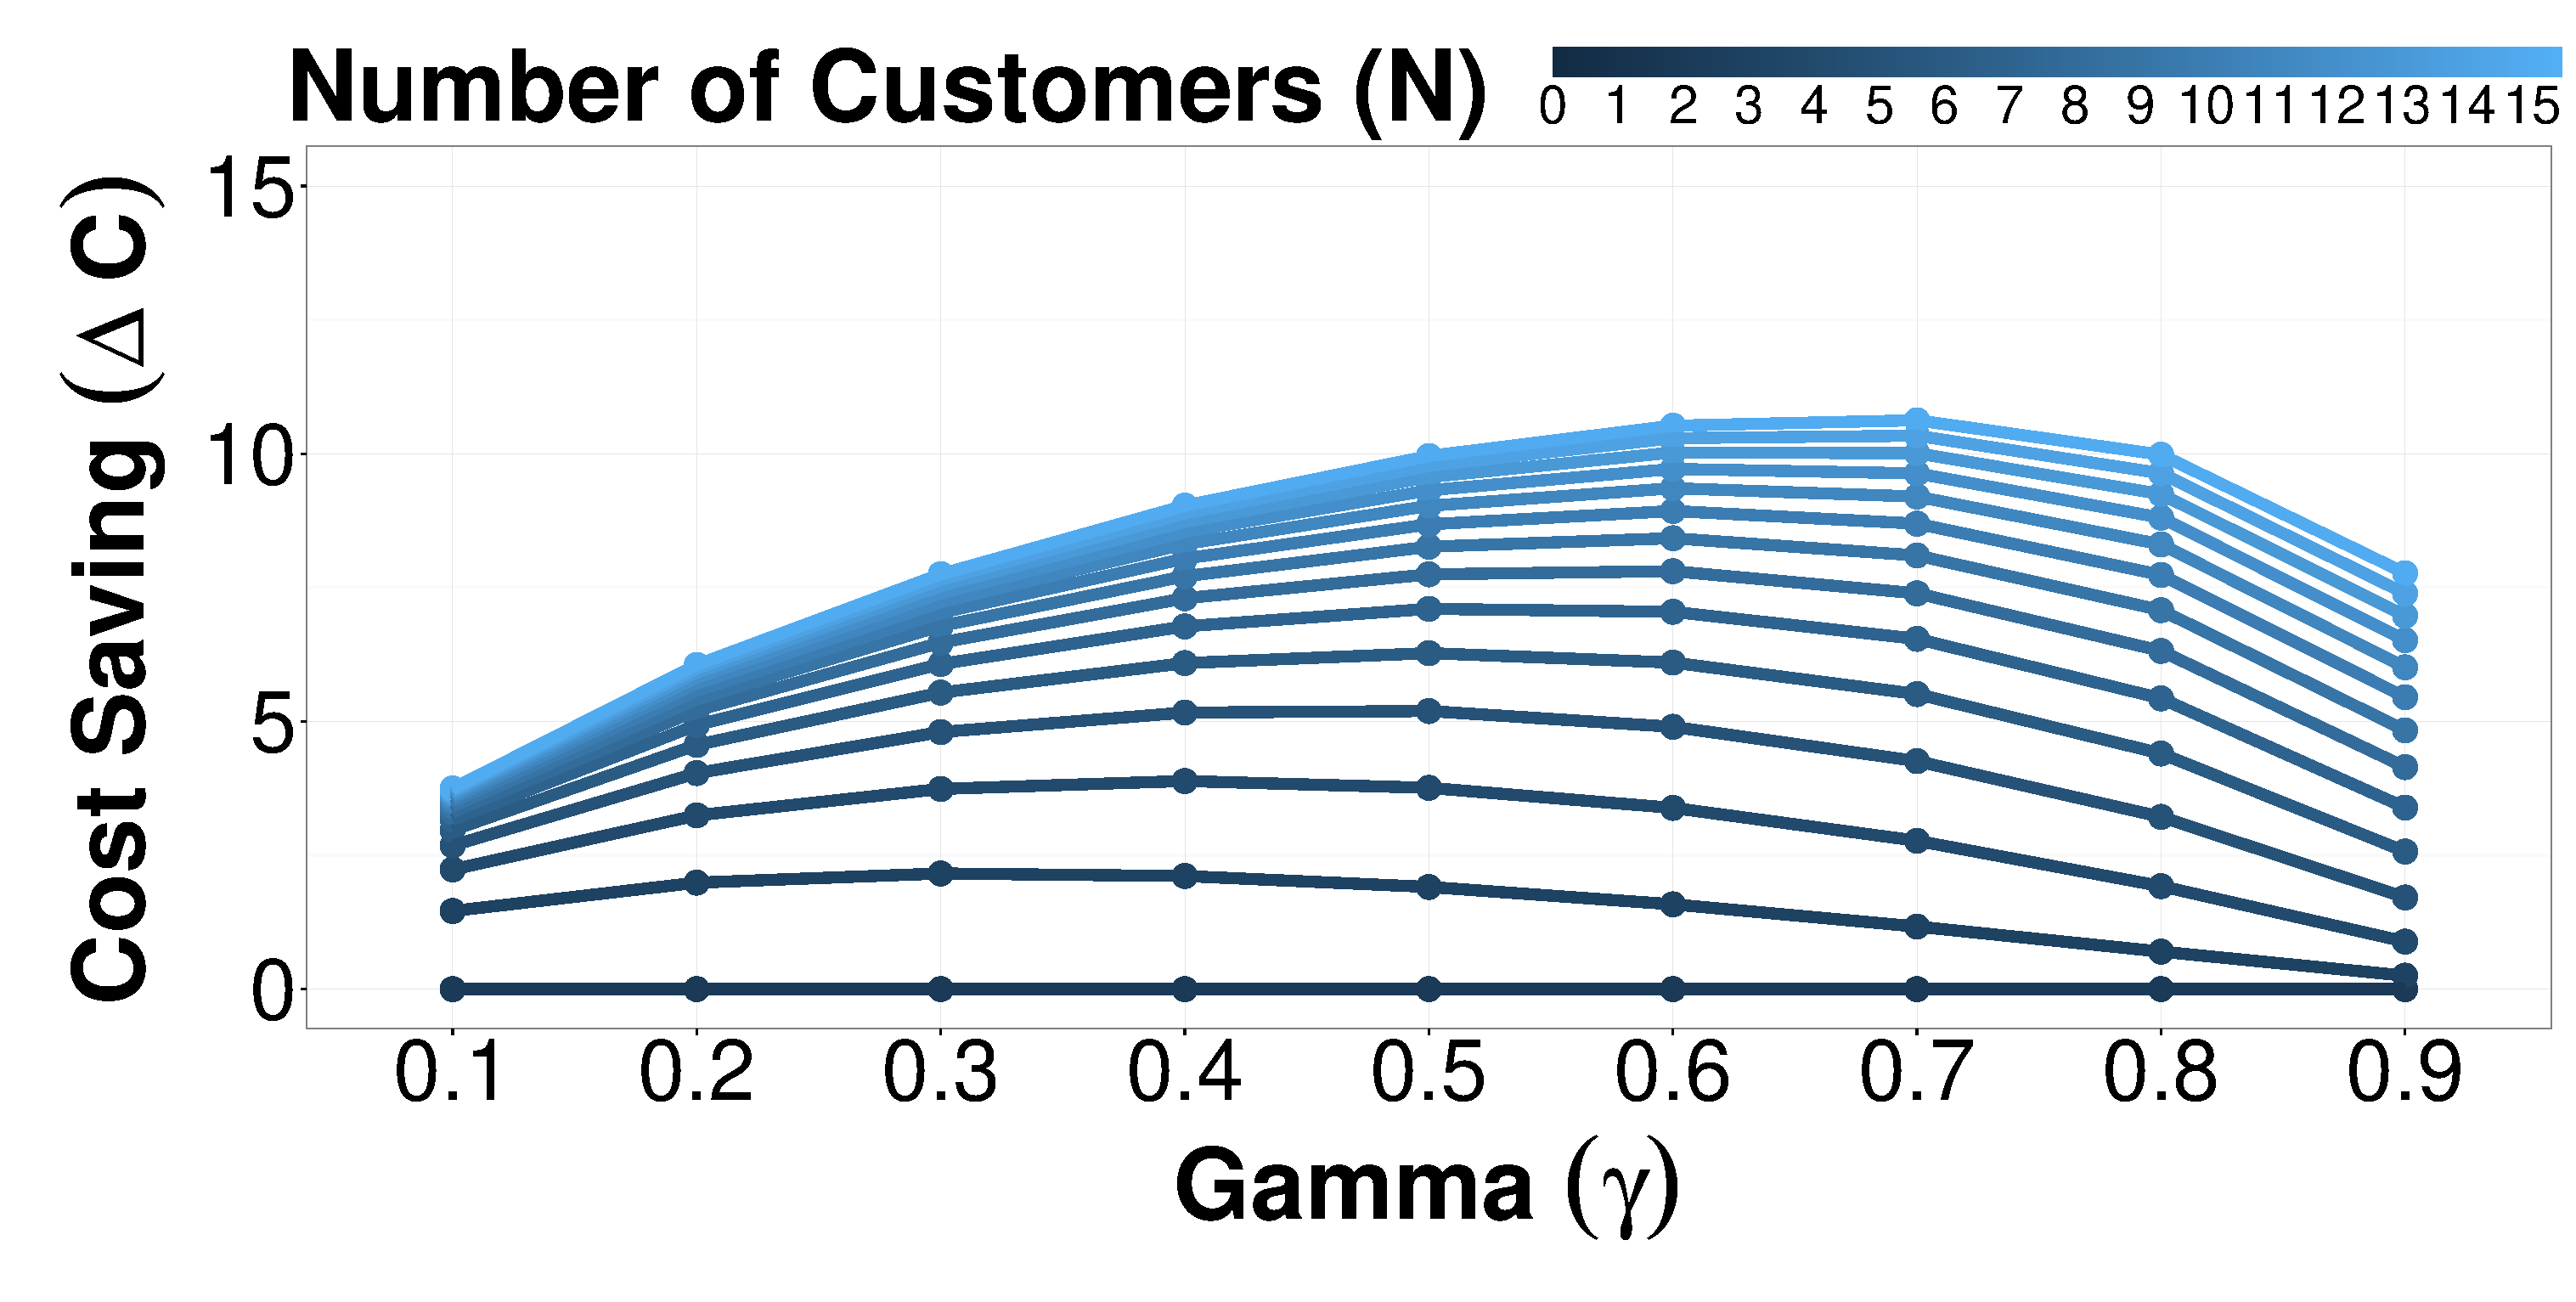
\includegraphics[width=0.85\textwidth]{Cost_Saving_Line_Num.eps}
	\end{figure}

	\begin{itemize}
		\item For fixed $\gamma$, $\Delta C$ increases as $N$ increases (at a decreasing rate)
		\item $\Delta C$ is at a minimum for the extreme values of $\gamma$ where one of the costs is heavily prioritised
	\end{itemize}
\end{frame}

\section{Simulation Studies}

\begin{frame}
	\frametitle{Simulation}

	\begin{itemize}
		\item Consider the problem of scheduling $15$ customers
		\item Assume $\mu = 1$ and $\gamma = 0.5$
		\item Expected cost of static schedule is $15.05$
		\item Expected cost of dynamic schedule is $13.55$
		\item Desire broader understanding of difference between schedules
		\item Simulate a million runs to compare schedule performance
	\end{itemize}
\end{frame}

\begin{frame}
	\frametitle{Schedule Cost}

	\begin{figure}
		\centering
		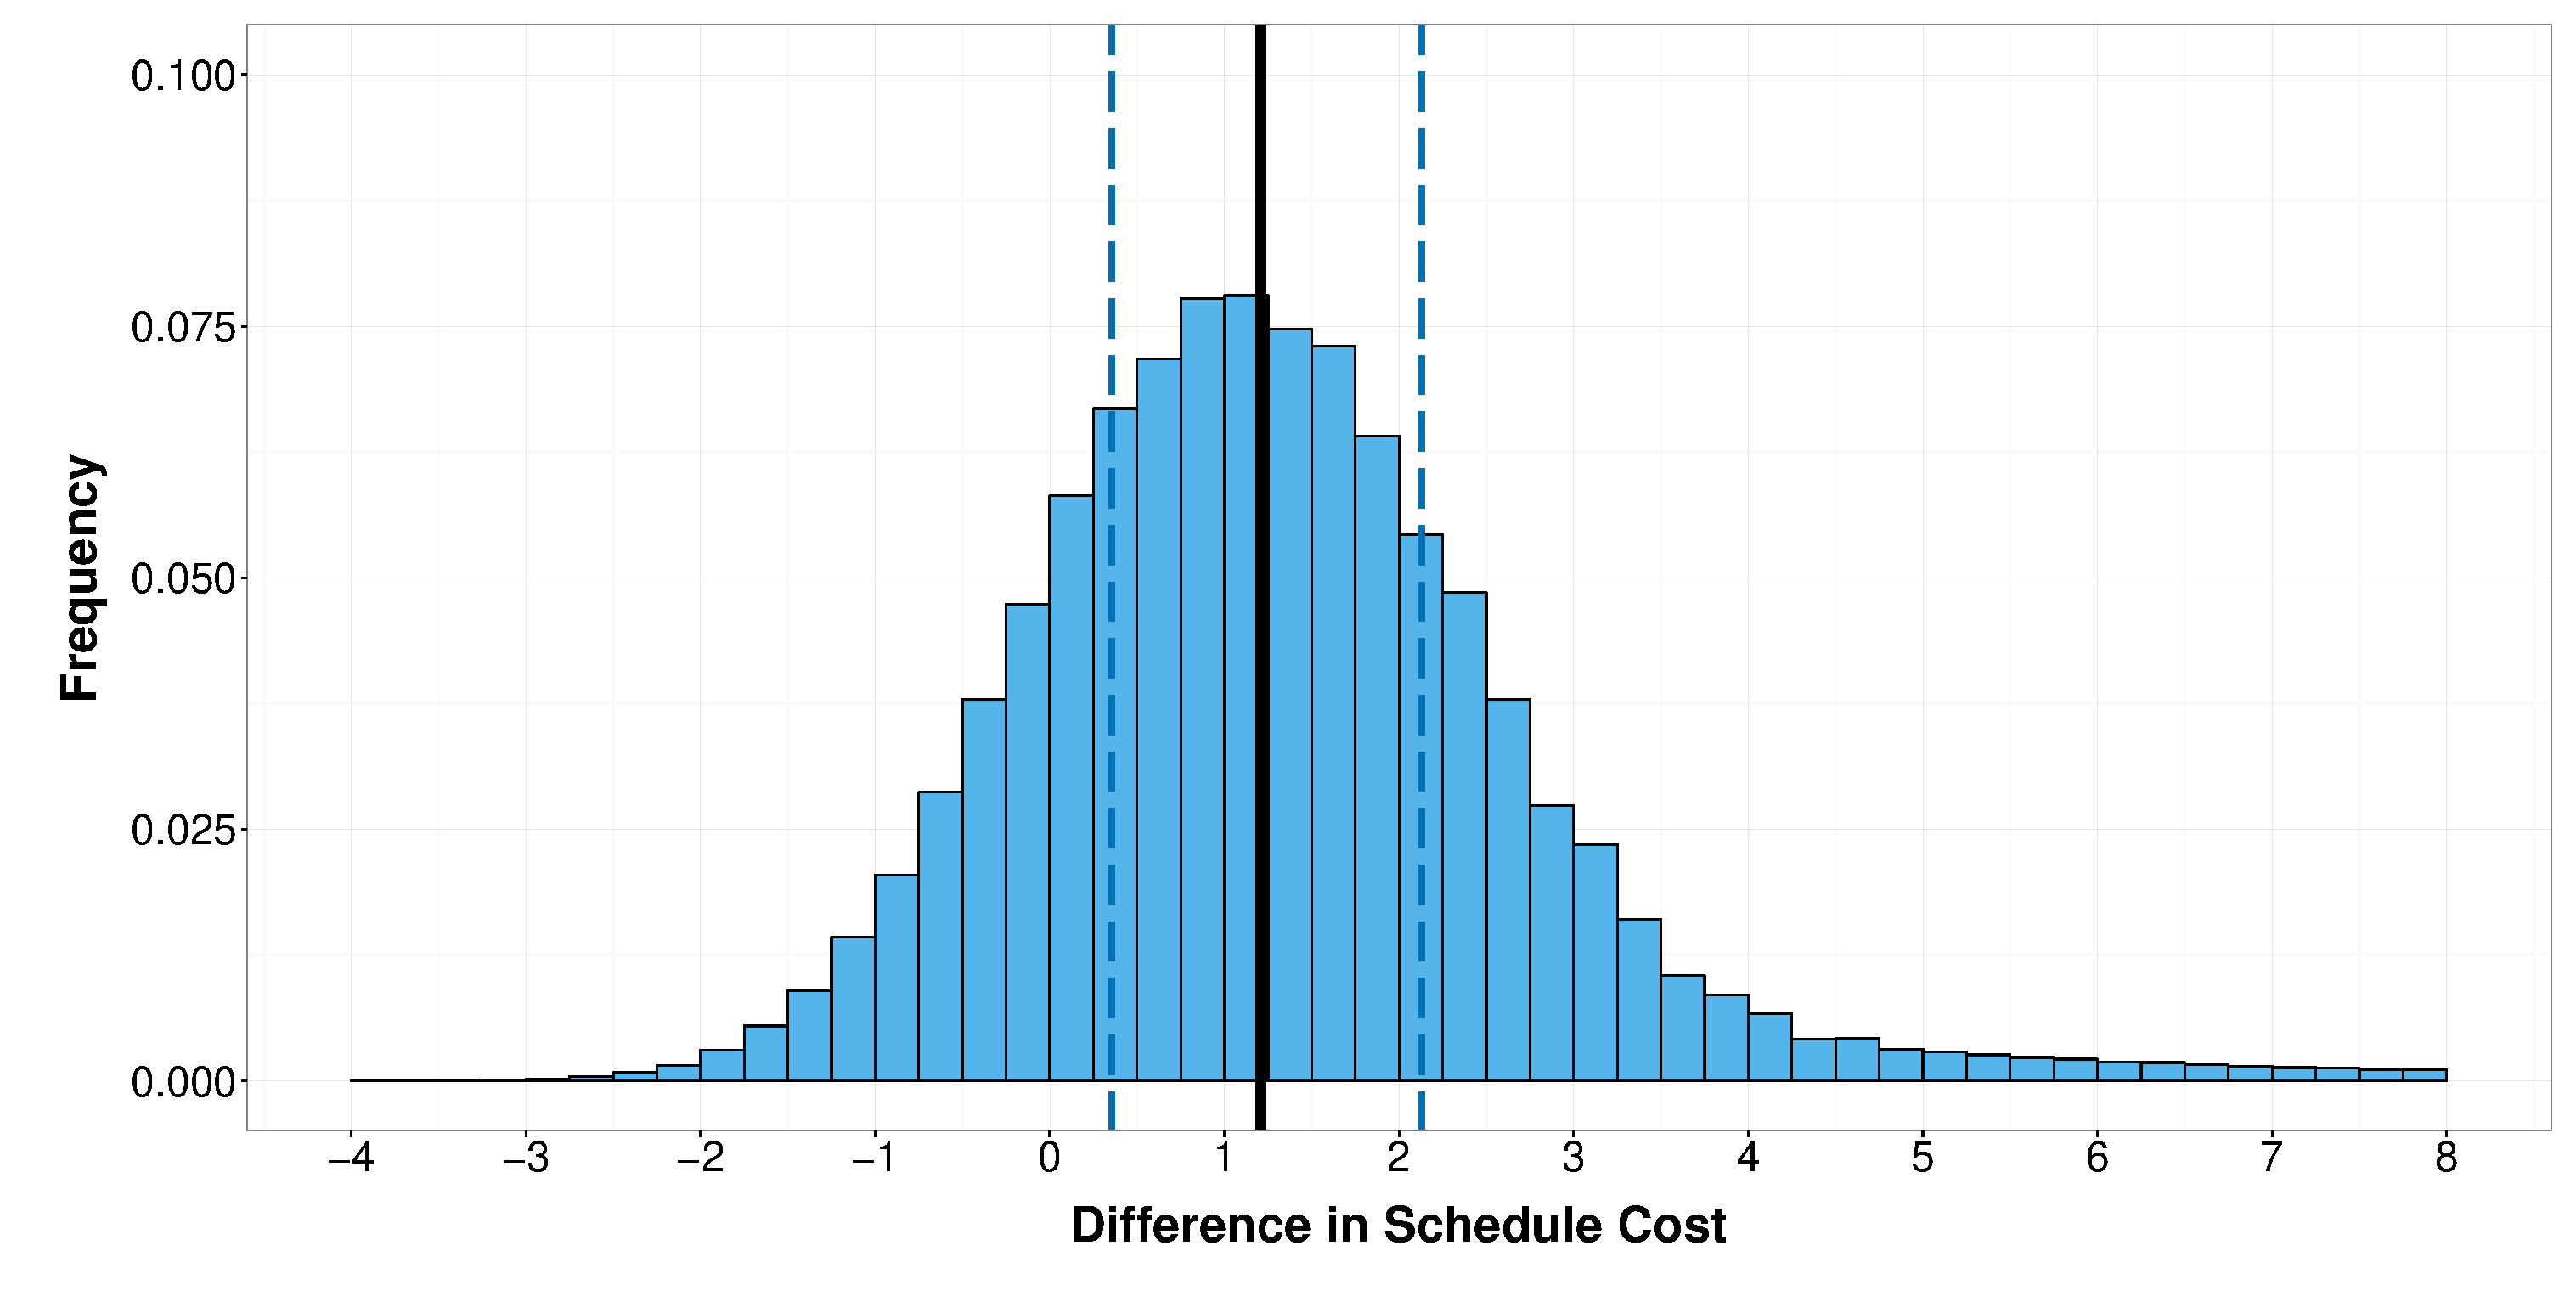
\includegraphics[width=0.85\textwidth]{Cost_Hist_Diff.eps}
	\end{figure}

	\begin{itemize}
		\item Static schedule outperforms the dynamic schedule for a proportion of the simulation runs
		\item For the majority of the runs, the static schedule has a considerably greater cost than the dynamic schedule
	\end{itemize}
\end{frame}

\begin{frame}
	\frametitle{Customer Arrival Times}

	\begin{figure}
		\centering
		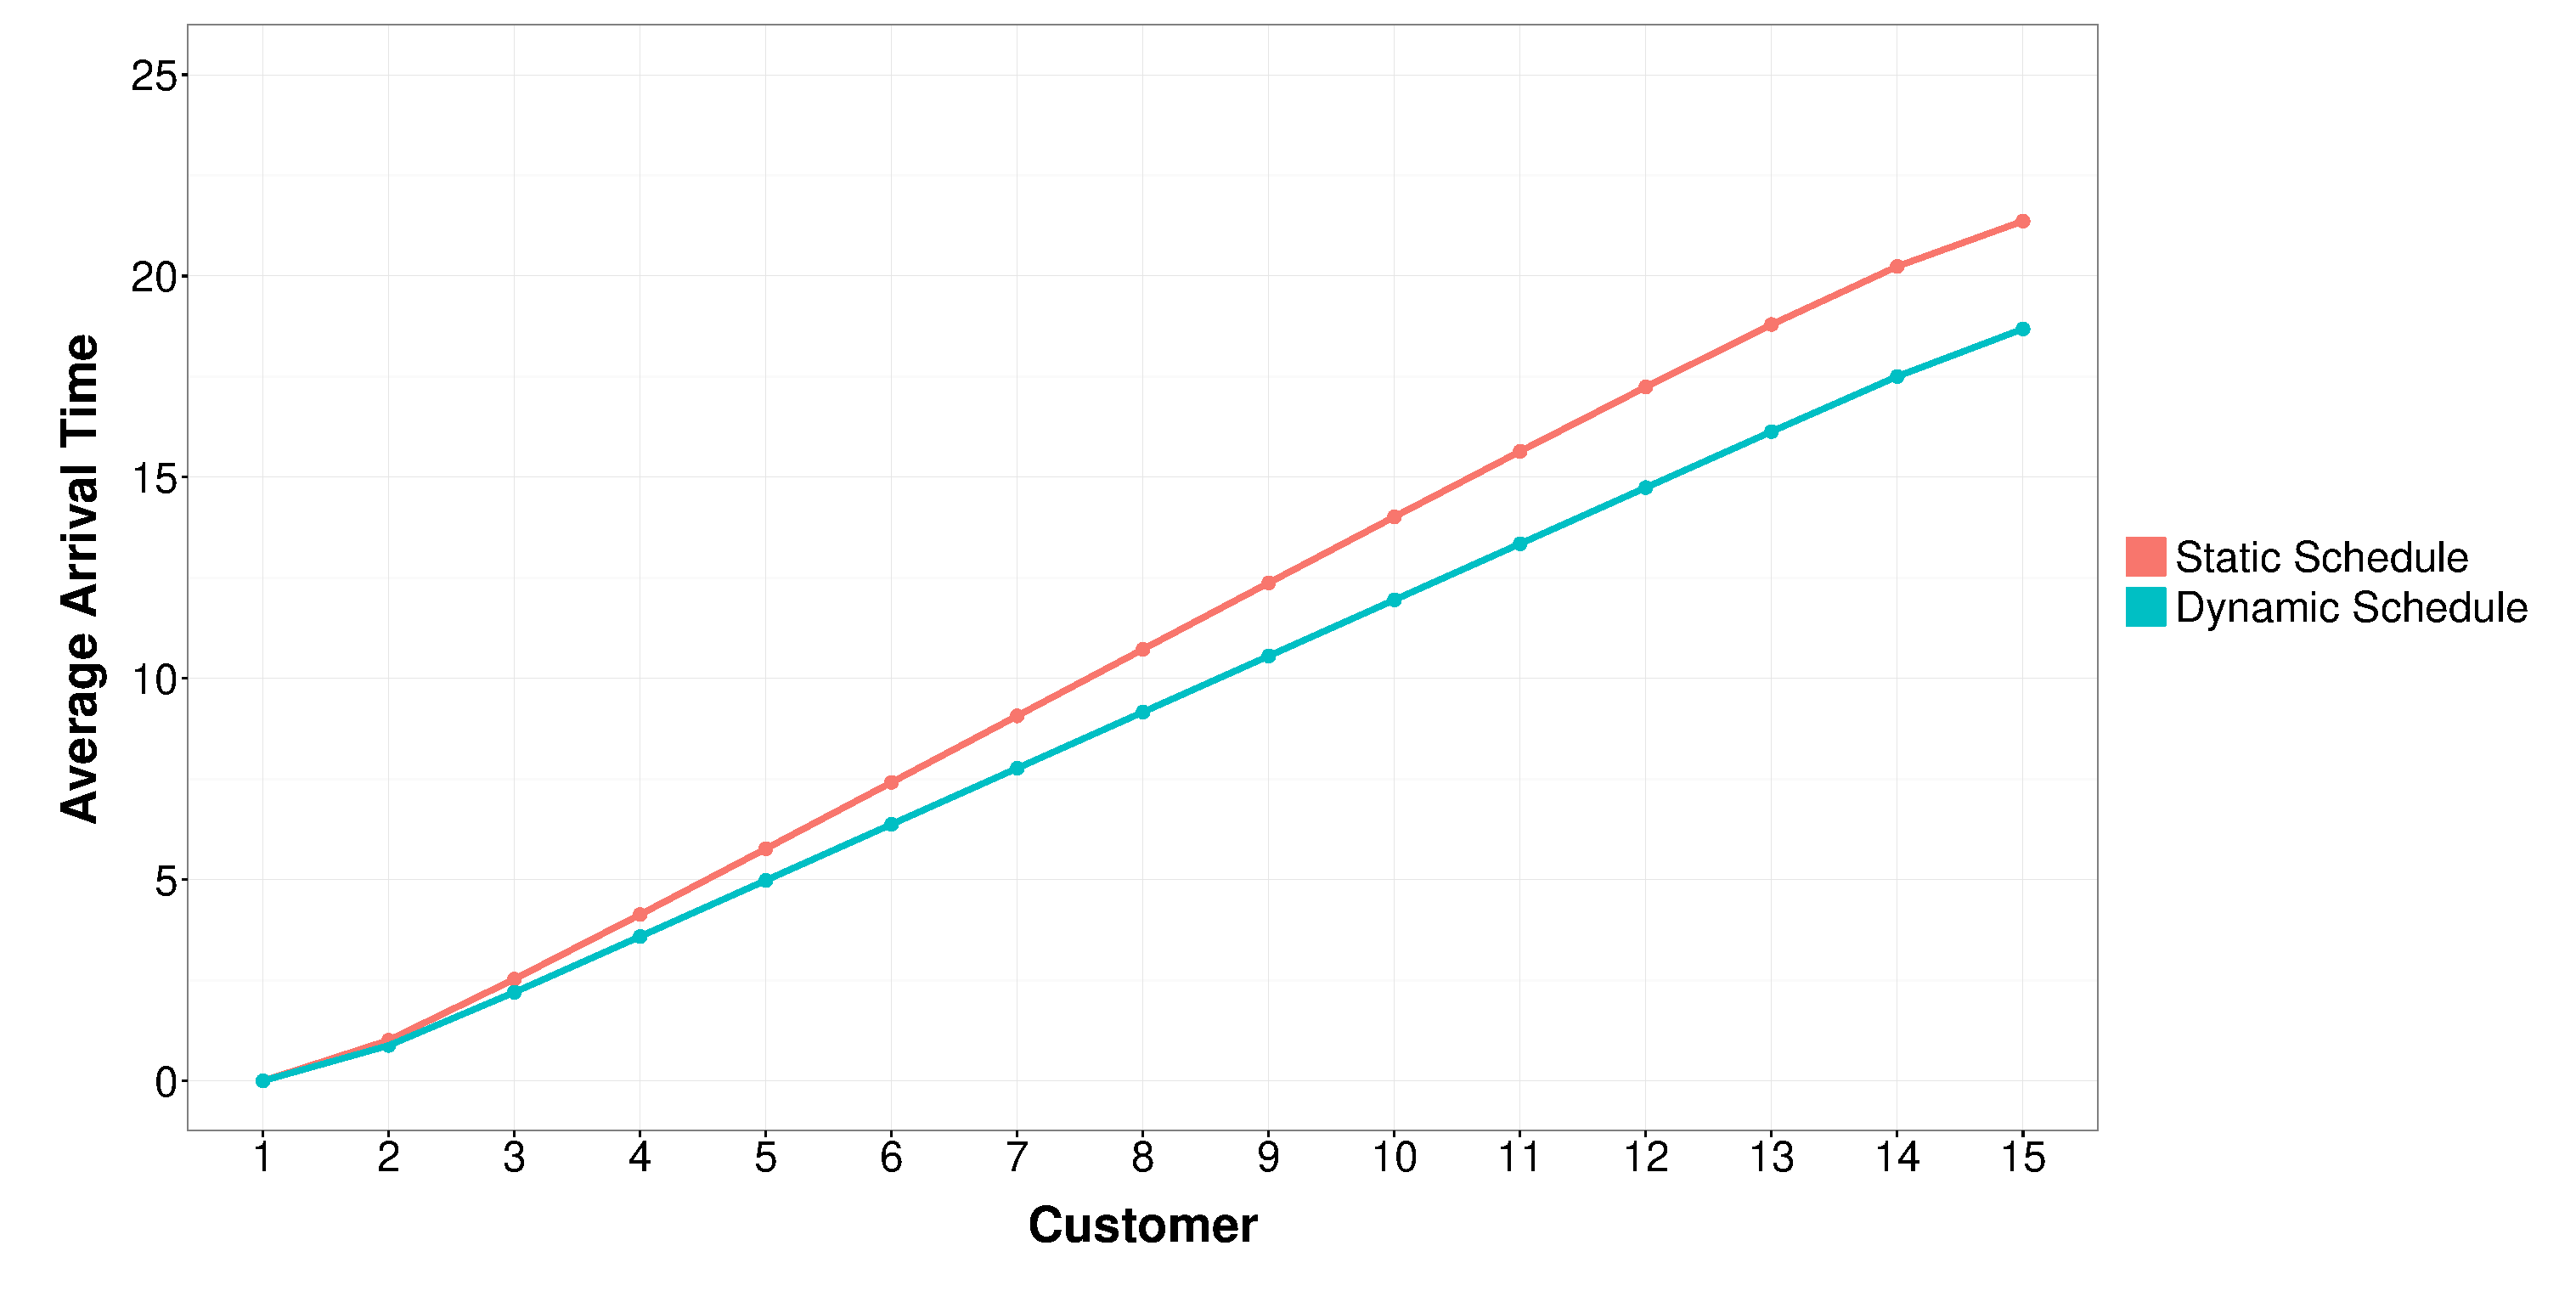
\includegraphics[width=0.85\textwidth]{AT_Line.eps}
	\end{figure}

	\begin{itemize}
		\item Mean arrival time is similar for first four or five customers
		\item Later customers arrive significantly earlier in dynamic schedule
	\end{itemize}
\end{frame}

\begin{frame}
	\frametitle{Mean Waiting Time}

	\begin{figure}
		\centering
		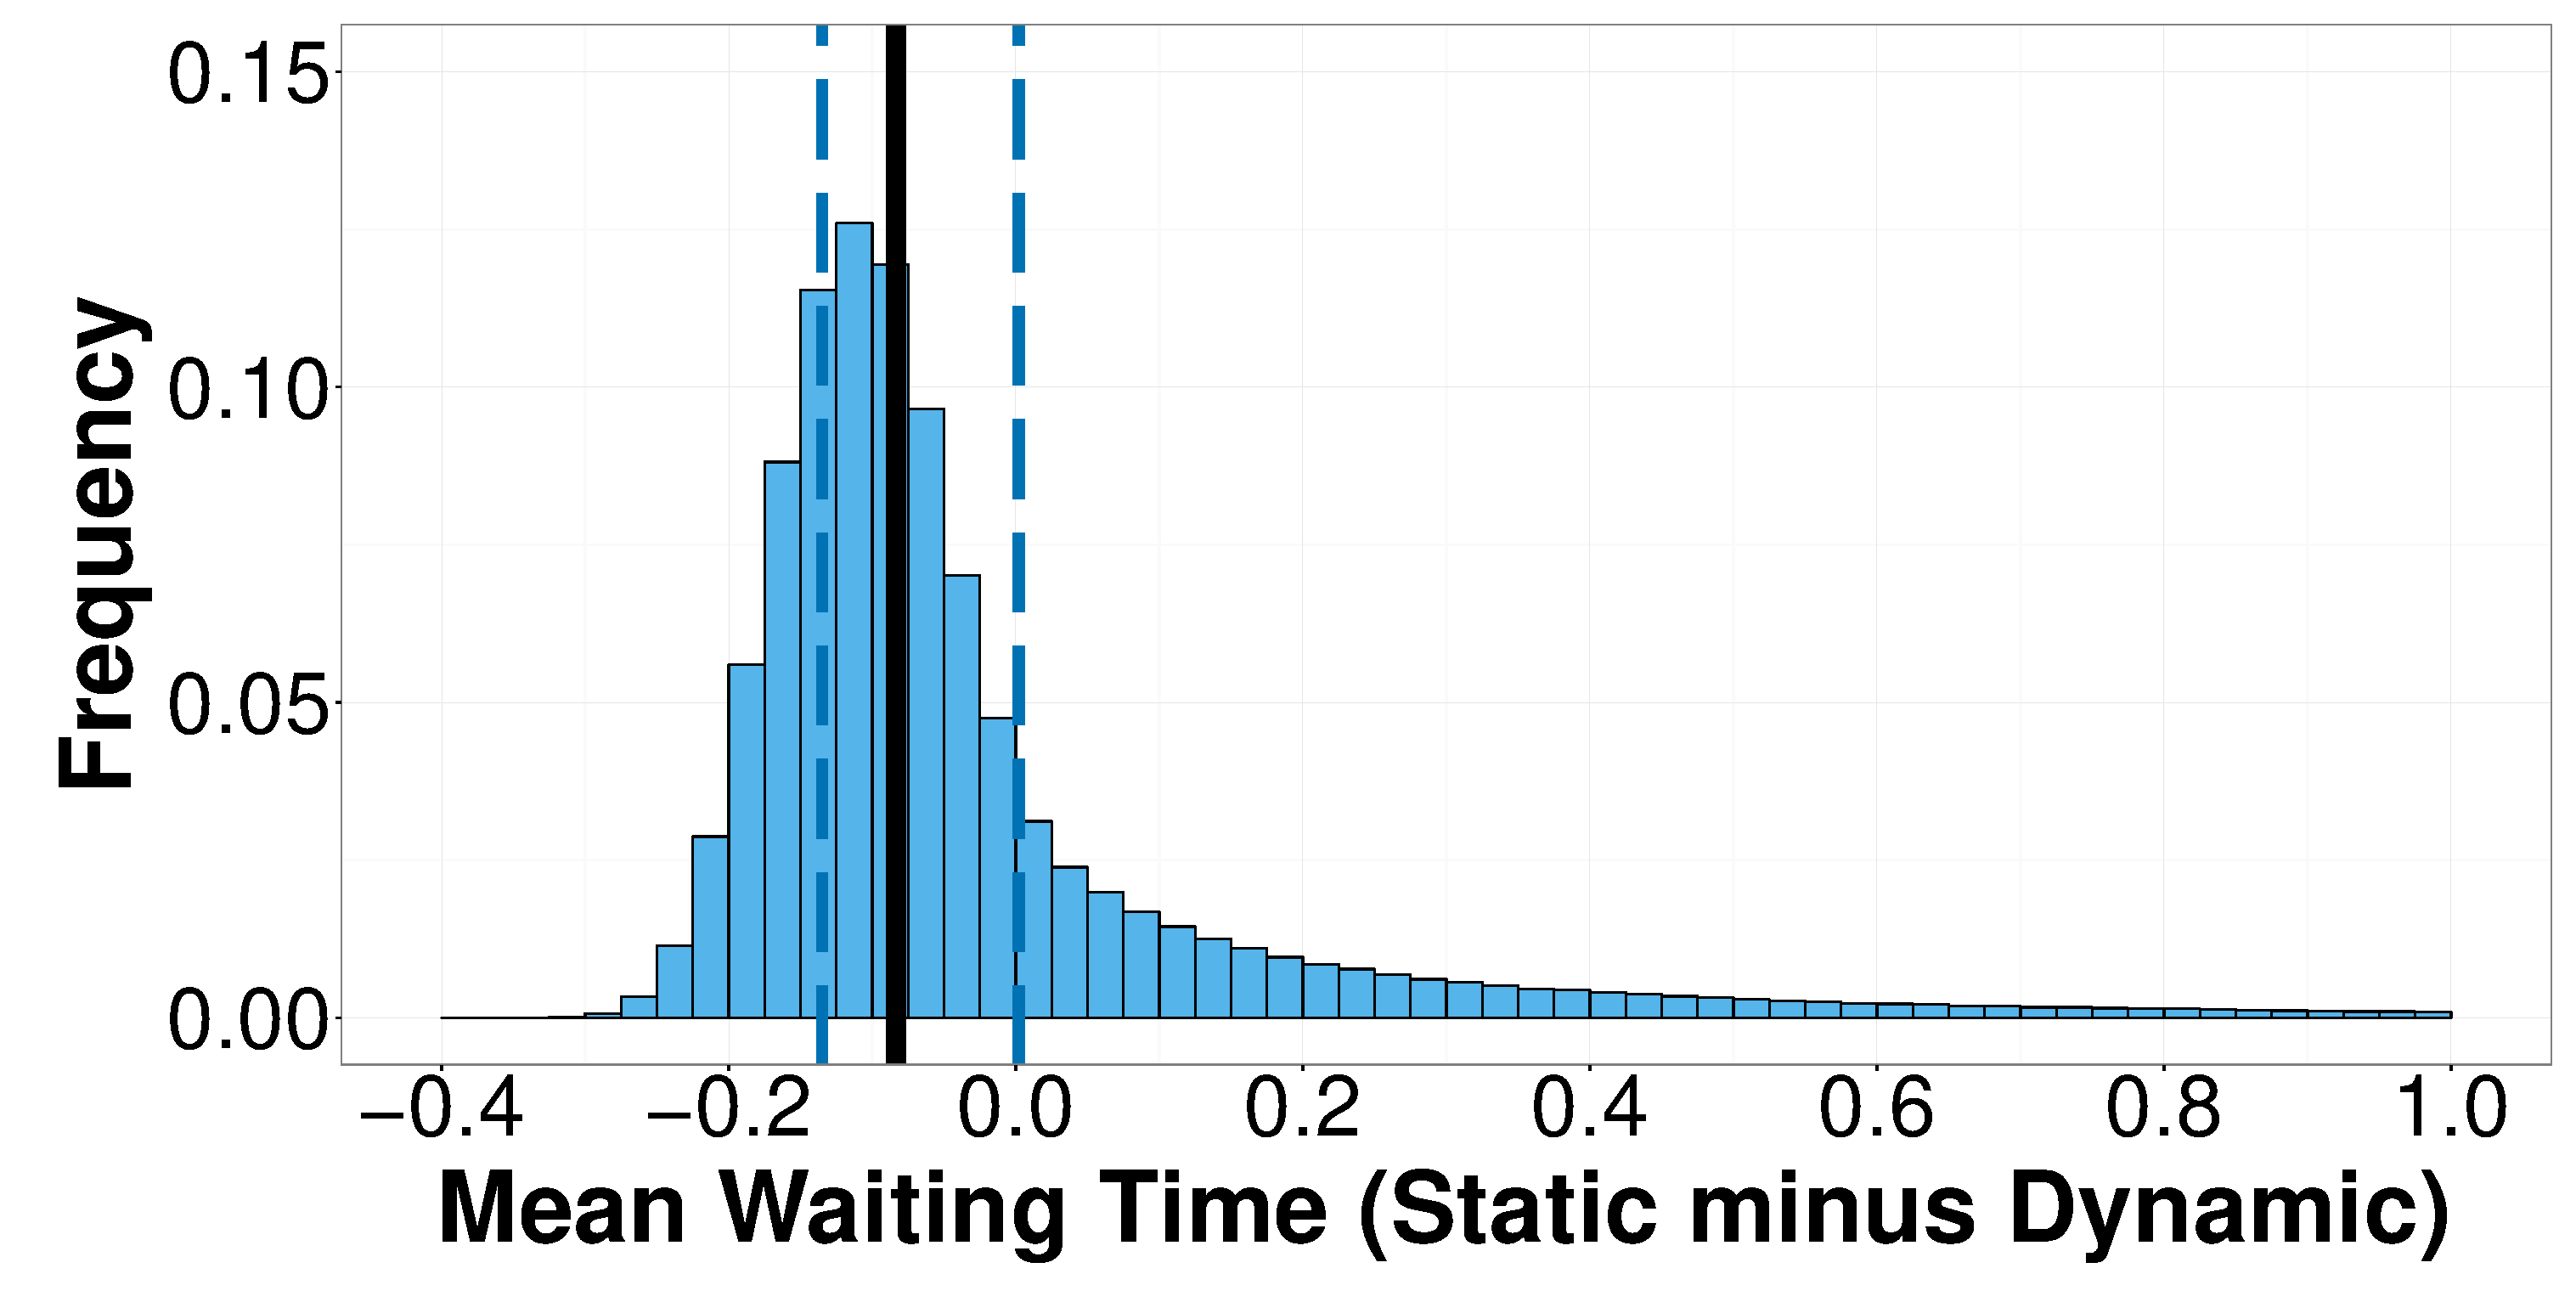
\includegraphics[width=0.85\textwidth]{WT_Hist_Diff.eps}
	\end{figure}

	\begin{itemize}
		\item For the majority of the runs, the customers in the static schedule have shorter mean waiting time
		\item Dynamic schedule is less prone to runs with extremely long waiting times
	\end{itemize}
\end{frame}

\begin{frame}
	\frametitle{Customer Waiting Times}

	\begin{figure}
			\centering
			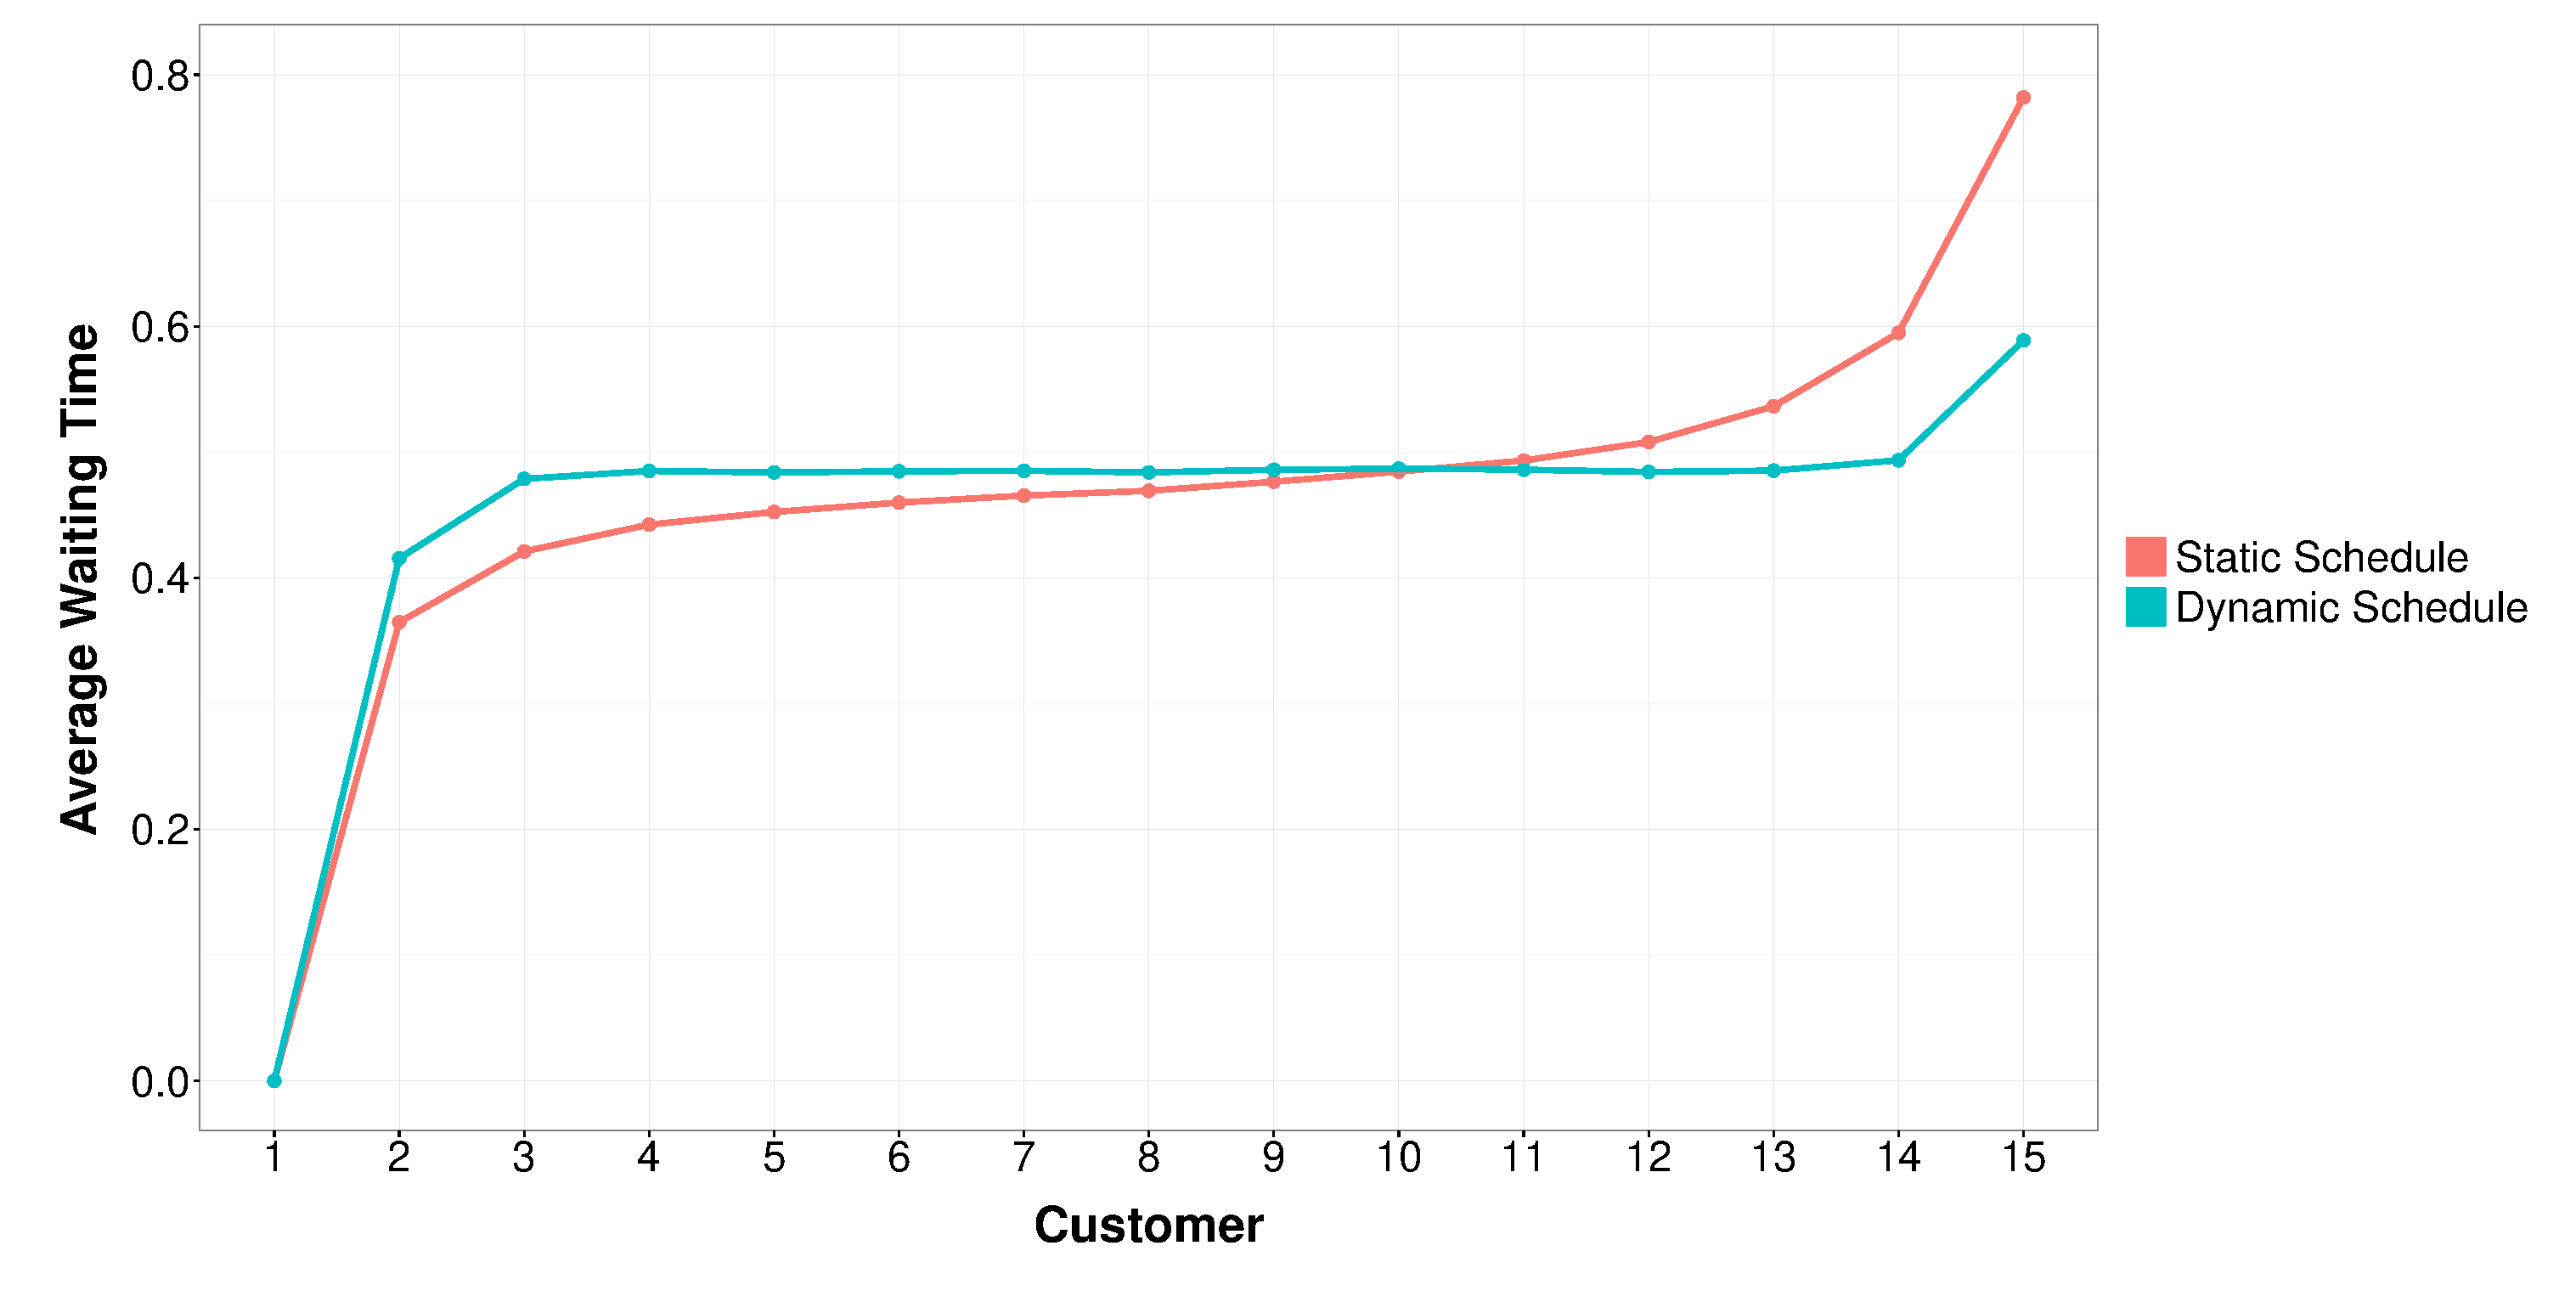
\includegraphics[width=0.85\textwidth]{WT_Line_Avg.eps}
	\end{figure}
		
	\begin{itemize}
		\item First few customers wait longer in the dynamic schedule, but last few customers wait longer in the static schedule
		\item Dynamic schedule is fairer
	\end{itemize}
\end{frame}

\begin{frame}
	\frametitle{Server Availability Time}

	\begin{figure}
		\centering
		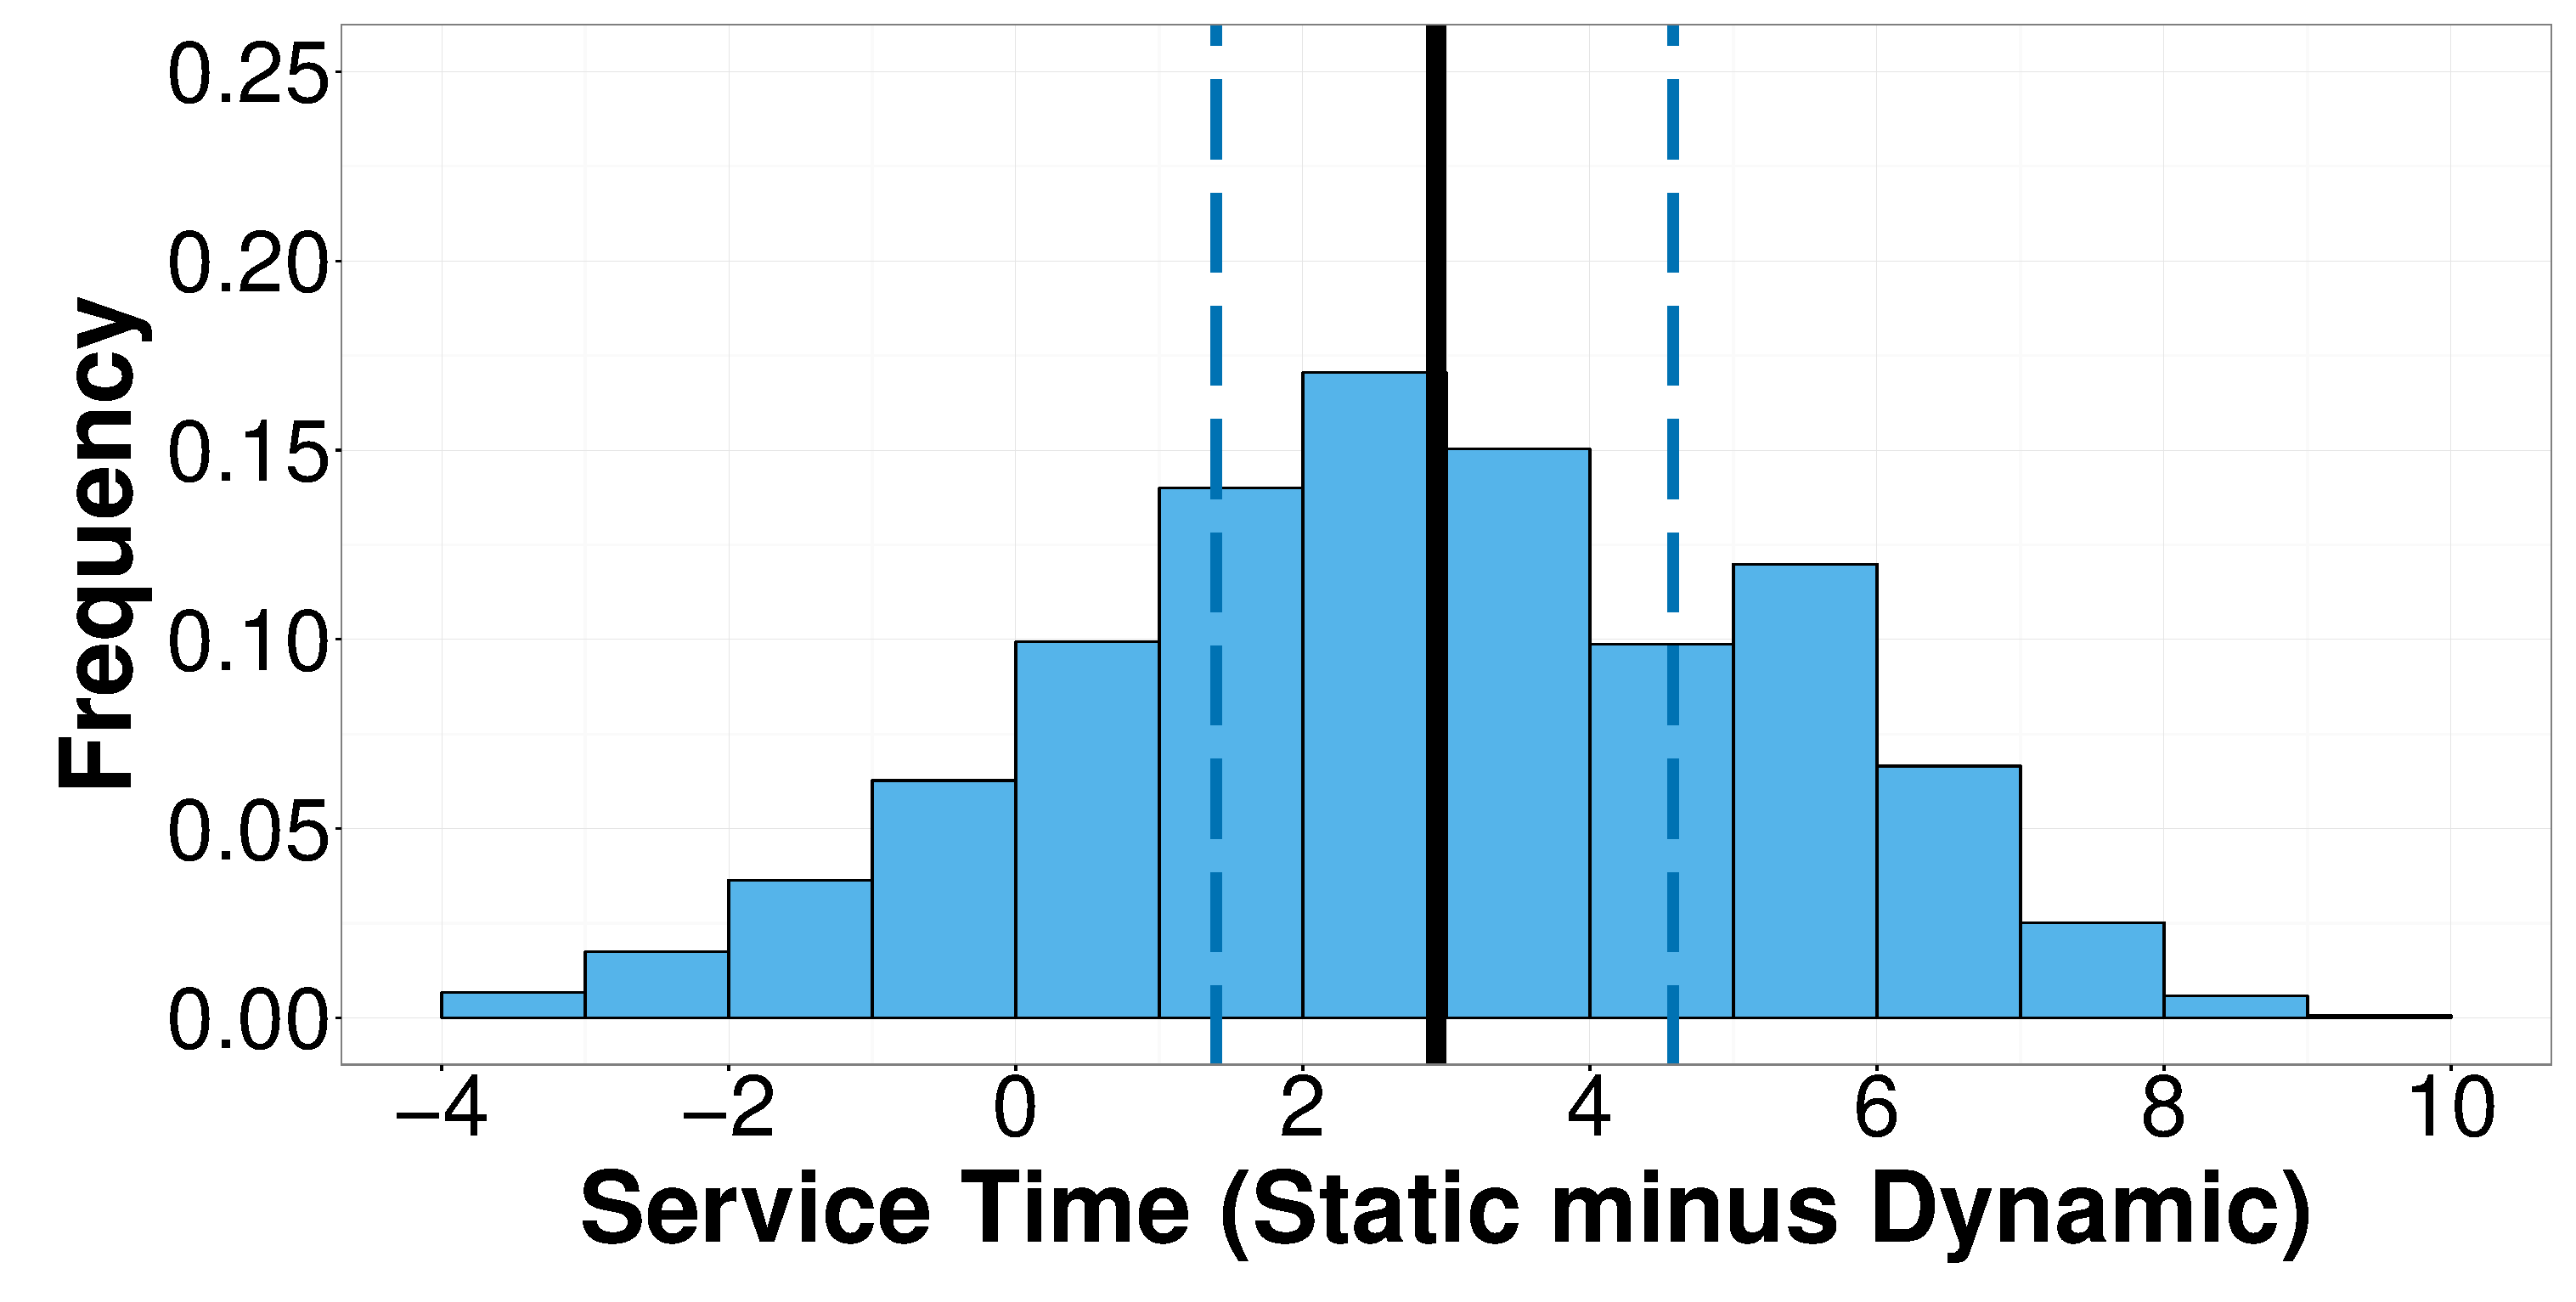
\includegraphics[width=0.85\textwidth]{TST_Hist_Diff.eps}
	\end{figure}

	\begin{itemize}
		\item Dynamic schedule has generally lower server availability time
		\item Static schedule is limited by fixed arrival time of last customer
	\end{itemize}
\end{frame}

\section{Conclusion}

\begin{frame}
	\frametitle{Conclusion}

	\begin{itemize}
		\item Dynamic schedules often significantly outperform static schedules
		\item Dynamic schedules are able to adapt during service, thus less prone to runs with extremely high cost
		\item Possible extensions:
		\begin{itemize}
			\item Minimum notice period
			\item Server's idle time in objective function
			\item Possibility of customer arriving late or not at all
		\end{itemize}
	\end{itemize}
\end{frame}

\appendix

\section{References}

\begin{frame}[allowframebreaks]
	\frametitle{References}
	\printbibliography[heading=none]
\end{frame}

\end{document}









































